\documentclass[UTF8,a4paper,12pt]{ctexbook} 

 \usepackage{graphicx}%学习插入图
 \usepackage{verbatim}%学习注释多行
 \usepackage{booktabs}%表格
 \usepackage{geometry}%图片
 \usepackage{amsmath}
 \usepackage{amssymb}
 \usepackage{listings}%代码
 \usepackage{xcolor}  %颜色
 \usepackage{enumitem}%列表格式
 \usepackage{tcolorbox}
 \usepackage{algorithm}  %format of the algorithm
 \usepackage{algorithmic}%format of the algorithm
 \usepackage{multirow}   %multirow for format of table
 \usepackage{tabularx} 	%表格排版格式控制
 \usepackage{array}	%表格排版格式控制
 \usepackage{hyperref} %超链接 \url{URL}
\CTEXsetup[format+={\flushleft}]{section}


\geometry{left=1.6cm,right=1.8cm,top=2cm,bottom=1.7cm} %设置文章宽度

\pagestyle{plain} 		  %设置页面布局
\author{\kaishu 郑华}
\title{\textbf{C++ 设计模式23种}}
 %代码效果定义
 \definecolor{mygreen}{rgb}{0,0.6,0}
 \definecolor{mygray}{rgb}{0.5,0.5,0.5}
 \definecolor{mymauve}{rgb}{0.58,0,0.82}
 \lstset{ %
 	backgroundcolor=\color{white},   % choose the background color
 	basicstyle=\footnotesize\ttfamily,        % size of fonts used for the code
 	%stringstyle=\color{codepurple},
 	%basicstyle=\footnotesize,
 	%breakatwhitespace=false,         
 	%breaklines=true,                 
 	%captionpos=b,                    
 	%keepspaces=true,                 
 	%numbers=left,                    
 	%numbersep=5pt,                  
 	%showspaces=false,                
 	%showstringspaces=false,
 	%showtabs=false,        
 	columns=fullflexible,
 	breaklines=true,                 % automatic line breaking only at whitespace
 	captionpos=b,                    % sets the caption-position to bottom
 	tabsize=4,
 	commentstyle=\color{mygreen},    % comment style
 	escapeinside={\%*}{*)},          % if you want to add LaTeX within your code
 	keywordstyle=\color{blue},       % keyword style
 	stringstyle=\color{mymauve}\ttfamily,     % string literal style
  	frame=single,					%tb top and bottom; L left double line
  	xleftmargin=.06\textwidth, 
  	%xrightmargin=.1\textwidth,
 	rulesepcolor=\color{red!20!green!20!blue!20},
 	% identifierstyle=\color{red},
 	language=c++,
 }
\begin{document}          %正文排版开始
	\maketitle
	\tableofcontents
	
\chapter{创建型模式-5种}
\section{*单例模式-对象性能}
	\subsection{概要}
		通过单例模式可以\textbf{保证系统中一个类只有一个实例}而且该实例易于外界访问,从而方便\textbf{对实例个数的控制并节约系统资源}
		
		Singleton模式是设计模式中最为简单、最为常见、最容易实现,也是\textbf{最应该熟悉和掌握的模式}
		
		我们怎样去创建一个唯一的变量(对象)?\textit{在面向对象和面向过程结合的设计范式(如C++中)中},我们\textbf{可以通过一个全局变量实现这一点}。但是当我们遇到了\textit{纯粹的面向对象范式中},这一点可能就\textbf{只能是通过Singleton模式来实现了}
		
		Singleton 的典型结构图如下图\ref{singleton}:
		\begin{figure}[h]
			\centering
			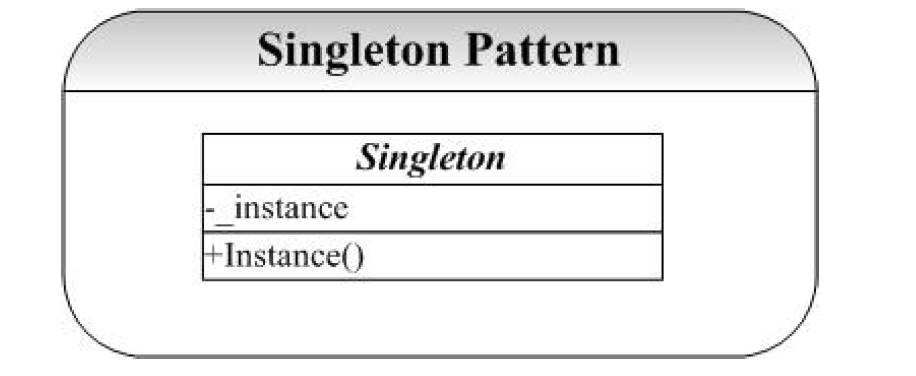
\includegraphics[width = 9cm]{Singleton.png}
			\caption{Singleton Pattern}
			\label{singleton}
		\end{figure}	
	\subsection{实现}
\begin{lstlisting}
////////////////////////////////Header File////////////////////////////////////
	#include <iostream> using namespace std;
			
	class Singleton
	{ 
	public: 
		static Singleton* Instance();
	protected:
		Singleton();
	private: 
		static Singleton* _instance;
	};
			
/////////////////////CPP File///////////////////////////////////////
	Singleton* Singleton::_instance = nullptr;  //静态成员需要在声明外进行初始化
	Singleton::Singleton() { cout<<"Singleton...."<<endl; }
	Singleton* Singleton::Instance() 
	{ 
		if (_instance == nullptr) 
		{ 
			_instance = new Singleton(); 
		}
	}
			
///////////////////Main File//////////////////////////////////////
	int main()
	{
		Singleton* sgn = Singleton::Instance();
		return 0;
	}
\end{lstlisting}
	
	\subsection{应用场景}
		Singleton模式在开发中经常用到,且不说我们开发过程中一些变量必须是唯一的,比如说打印机的实例等等。
		
		Singleton模式经常和Factory(AbstractFactory)模式在一起使用,\textbf{因为系统中工厂对象一般来说只要一个},因为系统我们就只要一个工厂来创建对象就可以了
\newpage
\section{*工厂模式 -对象创建}
	\subsection{简单工厂}
		一般只需要告诉工厂类所需要的类型,工厂类就会返回需要的产品类,但客户端看到的只是产品的抽象对象,无需关心到底是返回了哪个子类。客户端唯一需要知道的具体子类就是工厂子类。除了这点,基本是达到了依赖倒转原则的要求。
		
		我们不用工厂类,只用AbstractProduct和它的子类,那客户端每次使用不同的子类的时候都需要知道到底是用哪一个子类,当类比较少的时候还没什么问题,但是当类比较多的时候,管理起来就非常的麻烦了,就必须要做大量的替换,一个不小心就会发生错误。
		
		而使用了工厂类之后,就不会有这样的问题,不管里面多少个类,我只需要知道类型号即可。不过,这里还有一个疑问,那就是如果我每次用工厂类创建的类型都不相同,这样修改起来的时候还是会出现问题,还是需要大量的替换。所以简单工厂模式一般应该于程序中大部分地方都只使用其中一种产品,工厂类也不用频繁创建产品类的情况。这样修改的时候只需要修改有限的几个地方即可。
		
		Factory 的典型结构图如下图\ref{FactorySimple}:
		\begin{figure}[h]
			\centering
			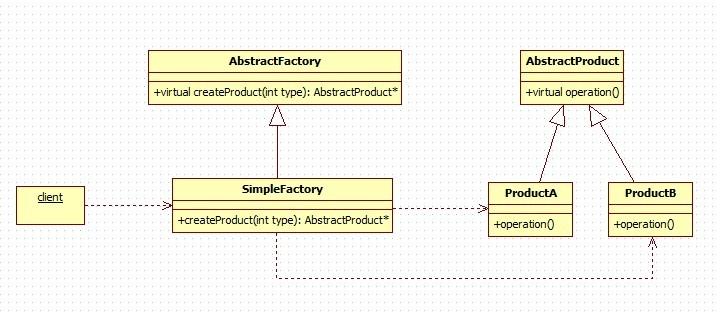
\includegraphics[width = 14cm]{FactorySimple.jpg}
			\caption{Factory Pattern}
			\label{FactorySimple}
		\end{figure}
	\subsection{实现}	
\begin{lstlisting}
///////////////////////////Client//////////////////////////////////
	int main(){
		AbstractFactory* factory = new SimpleFactory();
		AbstractProduct* product = factory->createProduct(1);
		product->operation();
		delete product;
		product = nullptr;
	
		product = factory->createProduct(2);
		product->operation();
		delete product;
		product = nullptr;
		
		return 0;
	}
\end{lstlisting}
	\subsection{概要}
		工厂模式基本与\textbf{简单工厂模式}差不多,-\textit{每次添加一个产品子类都必须在工厂类中添加一个判断分支},这样违背了开放-封闭原则,因此,\textbf{工厂模式就是为了解决这个问题而产生的}。
		
		为了提高内聚(Cohesion)和松耦合(Coupling),我们经常会抽象出一些类的公共接口以形成抽象基类或者接口。这样我们可以通过声明一个指向基类的指针来指向实际的子类实现,达到了多态的目的。这里很容易出现的一个问题n多的子类继承自抽象基类,我们不得不在每次要用到子类的地方就编写诸如new ×××;的代码

		还有一种情况就是在父类中并不知道具体要实例化哪一个具体的子类
		
		以上两个问题也就\textbf{引出了Factory模式的两个最重要的功能}:
			\begin{itemize}[itemindent = 1em]
				\item 定义创建对象的接口,封装了对象的创建
				
				\item 使得\textbf{具体化类的工作延迟到了子类中}
				
				\item 客户端基本\textbf{不用关心使用的是哪个产品},只需要知道用\textbf{哪个工厂}就行了
			\end{itemize}
			
		Factory 的典型结构图如下图\ref{Factory}:
		\begin{figure}[h]
			\centering
			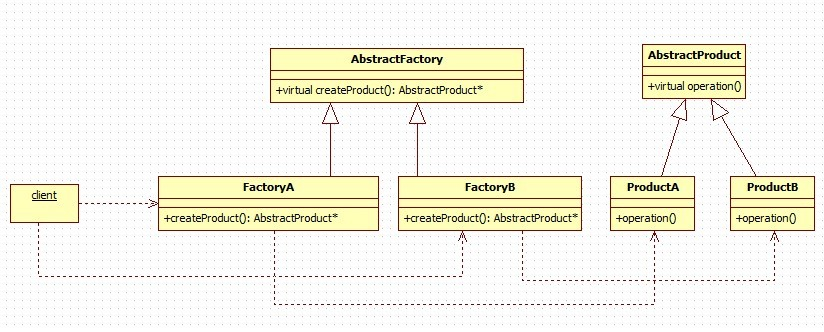
\includegraphics[width = 14cm]{Factory.jpg}
			\caption{Factory Pattern}
			\label{Factory}
		\end{figure}
	\subsection{实现}
\begin{lstlisting}
//////////////AbstractProduct with ConcreteProduct////////////////
	class AbstractProduct{
	public:
		AbstractProduct();
		virtual ~AbstractProduct();
	
	public:
		virtual void operation() = 0;
	};
	
	class ProductA:public AbstractProduct{
	public:
		ProductA();
		virtual ~ProductA();
	
	public:
		void operation() override;
	};
	
	class ProductB:public AbstractProduct{
	public:
		ProductB();
		~ProductB();
	
	public:
		void operation() override;
	};
//////////////////AbstractFactory with ConcreteFactory////////////
	class AbstractFactory{
	public:
		AbstractFactory();
		virtual ~AbstractFactory();
	
	public:
		virtual AbstractProduct* createProduct() = 0;    
	};
	
	class FactoryA:public AbstractFactory{
	public:
		FactoryA();
		~FactoryA();
	
	public:
		AbstractProduct* createProduct() override;
	};
	
	class FactoryB:public AbstractFactory{
	public:
		FactoryB();
		~FactoryB();
	
	public:
		AbstractProduct* createProduct() override;
	};
/////////////////////////Client///////////////////////////////////
	int main()
	{
		AbstractFactory* factory = new FactoryA();
		AbstractProduct* product = factory->createProduct();
		product->operation();
		delete product;
		product = nullptr;
		delete factory;
		factory = nullptr;
		
		factory = new FactoryB();
		product = factory->createProduct();
		product->operation();
		delete product;
		product = nullptr;
		delete factory;
		factory = nullptr;
		return 0;
	}
\end{lstlisting}
	
	\subsection{应用场景}
		例如部署多种数据库的情况,\textbf{可能在不同的地方要使用不同的数据库},此时\textit{只需要在配置文件中设定数据库的类型},\textbf{每次再根据类型生成实例},\textit{这样,不管下面的数据库类型怎么变化,在客户端看来都是只有一个AbstractProduct},使用的时候根本无需修改代码。提供的类型也可以用比较便于识别的字符串,这样不用记很长的类名,还可以保存为配置文件。
		
		这样,每次只需要修改配置文件和添加新的产品子类即可。
		
		\textbf{所以简单工厂模式一般应用于多种同类型类的情况},将这些类隐藏起来,再提供统一的接口,便于维护和修改。	
	
	\subsection{参考}
		\url{http://www.cnblogs.com/cxjchen/p/3143633.html}
\newpage
\section{*抽象工厂模式 -对象创建}
	\subsection{概要}
		抽象工厂模式就变得比工厂模式更为复杂,就像上面提到的缺点一样,工厂模式和简单工厂模式要求产品子类必须要是同一类型的,拥有共同的方法,这就限制了产品子类的扩展。于是为了更加方便的扩展,抽象工厂模式就将同一类的产品子类归为一类,让他们继承同一个抽象子类,我们可以把他们一起视作一组,然后好几组产品构成一族
		
		此时,客户端要使用时必须知道是哪一个工厂并且是哪一组的产品抽象类。每一个工厂子类负责产生一族产品,而子类的一种方法产生一种类型的产品。在客户端看来只有AbstractProductA和AbstractProductB两种产品,使用的时候也是直接使用这两种产品。而通过工厂来识别是属于哪一族产品。
		
		AbstractFactory 的典型结构图如下图\ref{AbstractFactory}:
		\begin{figure}[h]
			\centering
			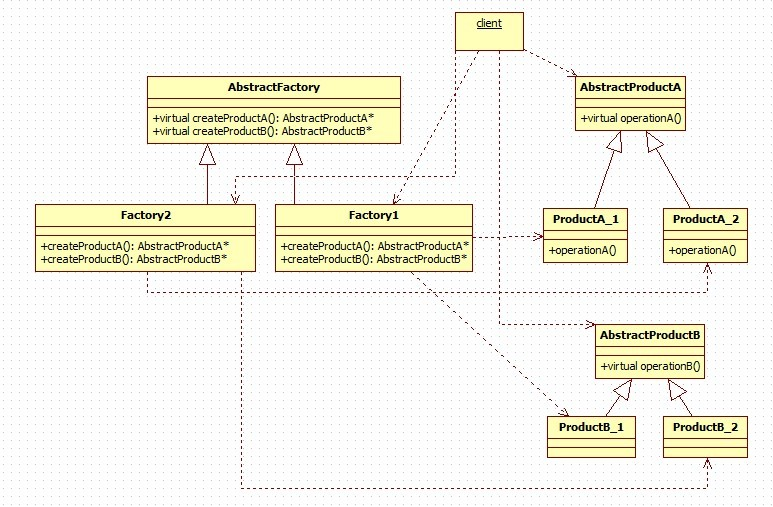
\includegraphics[width = 14cm]{AbstractFactory.jpg}
			\caption{AbstractFactory Pattern}
			\label{AbstractFactory}
		\end{figure}
		
		
		产品ProductA\_1和ProductB\_1构成一族产品,对应于有Factory1来创建,也就是说Factory1总是创建的ProductA\_1和ProductB\_1的产品,在客户端看来只需要知道是哪一类工厂和产品组就可以了。一般来说, ProductA\_1和ProductB\_1都是适应同一种环境的,所以他们会被归为一族。
		
		\textbf{特点}:
		\begin{itemize}
			\item 封装了产品的创建,使得不需要知道具体是哪种产品,只需要知道是哪个工厂就行了
			\item 可以支持不同类型的产品,使得模式灵活性更强
			\item 可以非常方便的使用一族中间的不同类型的产品
		\end{itemize}
	\subsection{实现}
\begin{lstlisting}
	int main()
	{
		AbstractFactory* factory = new Factory1();
		AbstractProductA* productA = factory->createProductA();
		AbstractProductB* productB = factory->createProductB();
		productA->operationA();
		productB->operationB();
		
		delete factory;
		factory = NULL;
		delete productA;
		productA = NULL;
		delete productB;
		productB = NULL;
		
		factory = new Factory2();
		productA = factory->createProductA();
		productB = factory->createProductB();
		productA->operationA();
		productB->operationB();
		
		delete factory;
		factory = NULL;
		delete productA;
		productA = NULL;
		delete productB;
		productB = NULL;
		return 0;
	}
\end{lstlisting}	
	
	
	\subsection{应用场景}
		例如Linux和windows\textbf{两种操作系统下},有2个挂件A和B,他们在Linux和Windows下面的实现方式不同,Factory1负责产生能在Linux下运行的挂件A和B,Factory2负责产生能在Windows下运行的挂件A和B,\textbf{这样如果系统环境发生变化了},我们\textbf{只需要修改工厂就行了}。
\newpage
\section{建造者模式 -对象创建}



\newpage
\section{原型模式 Prototype -对象创建}



\chapter{结构型模式-7种}
\section{桥接模式 Bridge - 单一职责}	
	\subsection{参考}
		http://www.cnblogs.com/houleixx/archive/2008/02/23/1078877.html	
	
	\subsection{概要}
		就拿汽车在路上行驶的来说。即有小汽车又有公共汽车,它们都不但能在市区中的公路上行驶,也能在高速公路上行驶。这你会发现,对于交通工具\textbf{(汽车)有不同的类型},然而它们所\textbf{行驶的环境(路)也在变化},在软件系统中就要\textbf{适应两个方面的变化}?怎样实现才能应对这种变化呢?
		
		在软件系统中,某些类型由于自身的逻辑,它具有两个或多个维度的变化,那么如何应对这种“多维度的变化”?如何利用面向对象的技术来使得该类型能够轻松的沿着多个方向进行变化,而又不引入额外的复杂度?这就要使用Bridge模式。
		
		\textbf{将抽象部分与实现部分分离,使它们都可以独立的变化}。
		
		Bridge 的典型结构图如下图\ref{Bridge}:
		\begin{figure}[h]
			\centering
			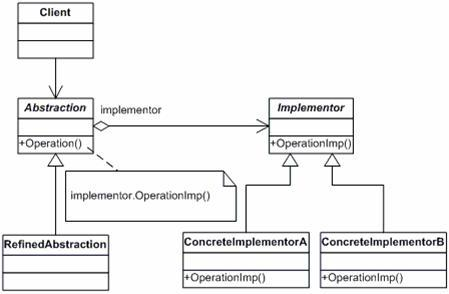
\includegraphics[scale= 0.8]{bridge.jpg}
			\caption{Bridge Pattern}
			\label{Bridge}
		\end{figure}
		
	
	\subsection{实现}	
		\subsubsection{传统实现}
		传统实现如图\ref{Bridge1}
		\begin{figure}[h]
			\centering
			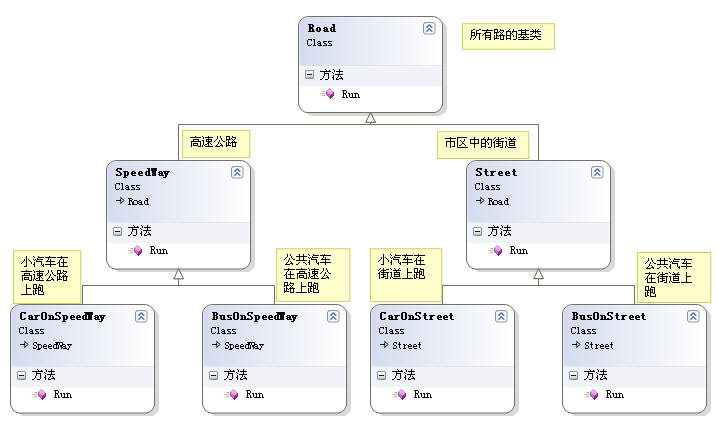
\includegraphics[scale= 0.8]{Bridge1.jpg}
			\caption{Normal Realize}
			\label{Bridge1}
		\end{figure}
		
		\subsubsection{桥接实现}
		桥接实现如\ref{Bridge2}
		\begin{figure}[h]
			\centering
			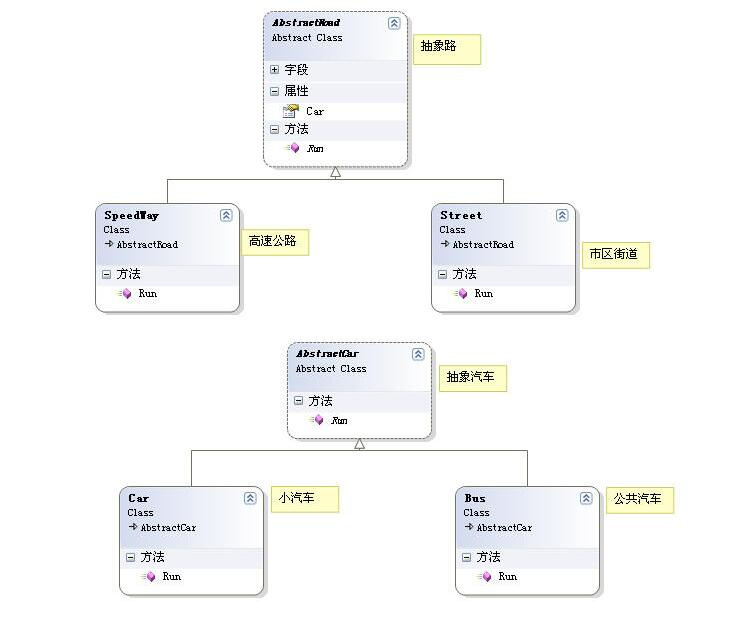
\includegraphics[scale= 0.8]{Bridge2.jpg}
			\caption{Bridge Realize}
			\label{Bridge2}
		\end{figure}
\begin{lstlisting}
	int Main()
	{
        //小汽车在高速公路上行驶;
        AbstractRoad Road1 = new SpeedWay();
	    Road1.Car = new Car();
	    Road1.Run();

	
	    //公共汽车在高速公路上行驶;
	    AbstractRoad Road2 = new SpeedWay();
	    Road2.Car = new Bus();
	    Road2.Run();
      }
\end{lstlisting}
		可以看到,\textbf{通过对象组合的方式},Bridge模式\textbf{把两个角色之间的继承关系改为了耦合的关系},从而\textbf{使}\textit{这两者可以从容自若的各自独立的变化},这也是Bridge模式的本意。	
		\begin{enumerate}
			\item Bridge模式使用“对象间的组合关系”解耦了抽象和实现之间固有的绑定关系,使得抽象和实现可以沿着各自的维度来变化。
			\item 所谓抽象和实现沿着各自维度的变化,即“子类化”它们,得到各个子类之后,便可以任意它们,从而获得不同路上的不同汽车
			\item Bridge模式有时候类似于多继承方案,但是多继承方案往往违背了类的单一职责原则(即一个类只有一个变化的原因),复用性比较差。Bridge模式是比多继承方案更好的解决方法
			\item Bridge模式的应用一般在“两个非常强的变化维度”,有时候即使有两个变化的维度,但是某个方向的变化维度并不剧烈——换言之两个变化不会导致纵横交错的结果,并不一定要使用Bridge模式
		\end{enumerate}
	\subsection{应用场景}
		\begin{itemize}
			\item 如果一个系统需要在构件的抽象化角色和具体化角色之间增加更多的灵活性,避免在两个层次之间建立静态的联系
			\item 设计要求实现化角色的任何改变不应当影响客户端,或者说实现化角色的改变对客户端是完全透明的。
			\item 一个构件有多于一个的抽象化角色和实现化角色,系统需要它们之间进行动态耦合。
			\item 虽然在系统中使用继承是没有问题的,但是由于抽象化角色和具体化角色需要独立变化,设计要求需要独立管理这两者
		\end{itemize}

	
\newpage
\section{装饰模式 Decorator- 单一职责}	


\newpage
\section{*组合模式 Composite -数据结构模式}	
	\subsection{概要}
		我们PC用到的文件系统,其实就是我们数据结构里的树形结构,\textbf{我们处理树中的每个节点时,其实不用考虑他是叶子节点还是根节点,因为他们的成员函数都是一样的,这个就是组合模式的精髓}。\textbf{他模糊了简单元素和复杂元素的概念,客户程序可以向处理简单元素一样来处理复杂元素},从而使得客户程序与复杂元素的内部结构解耦。
		
		将对象组合成树形结构以表示“部分-整体”的层次结构。组合模式使得用户对单个对象和组合对象的使用具有一致性。
		\textit{注明:树形结构里的叶子节点也有左右孩子,只不过他的孩子都是空}。
		
		\subparagraph{目的:}组合模式将对象组合成树形结构以表示“部分-整体”的层次结构[树状结构]。Composite\textbf{使得用户对\underline{单个对象}和\underline{组合对象}的使用具有一致性}。
		
		\subparagraph{结构:}Composite 的典型结构图如下图\ref{Composite}:
		\begin{figure}[h]
			\centering
			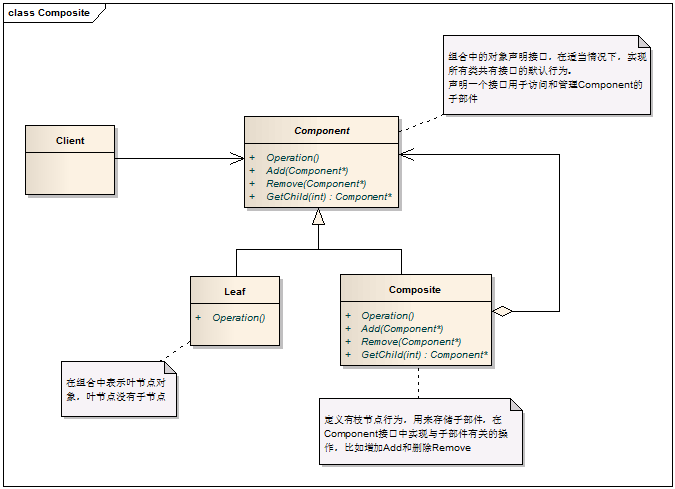
\includegraphics[scale= 0.8]{Composite.png}
			\caption{Composite Pattern}
			\label{Composite}
		\end{figure}
		
		\begin{enumerate}[itemindent = 1em]
			\item 抽象基类(Component-组件):在Component中声明所有用来管理子对象的方法,其中包括Add、Remove等,这样实现Component接口的所有子类都具备了Add和Remove。\textbf{这样做的好处就是叶节点和枝节点对于外界没有区别,它们具备 完全一致的行为 接口}。
			但问题也很明显,因为Leaf类本身不具备Add()、Remove()方法的 功能,所以实现它是没有意义的
			
			\item Component模式是为解决组件之间的递归组合提供了解决的办法,它主要分为两个派生类:
				\begin{enumerate}
					\item \textbf{不含有子组件的结点}:叶子结点 Leaf
					\item \textbf{含有子组件的节点}:Composite
				\end{enumerate}
		\end{enumerate}
	\subsection{实现}	
		\begin{lstlisting}
	
	/*
	Component抽象基类,为组合中的对象声明接口,声明了类共有接口的缺省行为(如这里的Add,Remove,GetChild函数),
	声明一个接口函数可以访问Component的子组件.
	*/
	class Component
	{
	public:
		//纯虚函数,只提供接口,没有默认的实现
		virtual void Operation()=0;    
		
		// 虚函数,提供接口,有默认的实现就是什么都不做
		virtual void Add(Component*);
		virtual void Remove(Component*);
		virtual Component* GetChild(int index);
		virtual ~Component();
		protected:
		Component();
	};
	
	//Leaf是叶子结点,也就是不含有子组件的结点类,所以不用实现Add、Remove、GetChild等方法
	class Leaf:public Component
	{
	public:
		//只实现Operation接口
		virtual void Operation();            
		Leaf();
		~Leaf();
	};
	
	//Composite:含有子组件的类
	class Composite:public Component
	{
	public:
		Composite();
		~Composite();
		//实现所有接口
		void Operation();
		void Add(Component*);
		void Remove(Component*);
		Component* GetChild(int index);
		private:
		//这里采用vector来保存子组件
		vector<Component*> m_ComVec;        
	};
	
	
///////////体现组合模式的MainClient///////////////////////

	
	int main()
	{
		/*
		不管是叶子Leaf还是Composite对象pRoot、pCom都实现了Operation接口,所以可以一致对待,直接调用Operation()
		体现了“使得用户对单个对象和组合对象的使用具有一致性。”
		*/
		Composite* pRoot = new Composite();
		
		//组合对象添加叶子节点
		pRoot->Add(new Leaf());
		
		Leaf* pLeaf1 = new Leaf();
		Leaf* pLeaf2 = new Leaf();
		
		//这里的叶子再添加叶子是没有意义的。
		//由于叶子与组合对象继承了相同的接口,所以语法上是对的,实际上什么也没做(继承自基类Component的Add方法)。
		//叶子节点只实现了Operation方法,其他Add、Remove、GetChild都继承自基类,没有实际意义。
		pLeaf1->Add(pLeaf2);
		pLeaf1->Remove(pLeaf2);
		//执行叶子Operation操作
		pLeaf1->Operation();
		
		//组合对象实现了基类Component的所有接口,所以可以做各种操作(Add、Remove、GetChild、Operation)。
		Composite* pCom = new Composite();
		//组合对象添加叶子节点
		pCom->Add(pLeaf1);
		//组合对象添加叶子节点
		pCom->Add(pLeaf2);
		//执行组合对象Operation操作
		pCom->Operation();
		
		//组合对象添加组合对象
		pRoot->Add(pCom);
		
		//执行组合对象Operation操作
		pRoot->Operation();
		
		//Component* cp = pCom->GetChild(0);
		//cp->Operation();
		
		//pCom->Remove(pLeaf1);
		
		return 0;
	}
		\end{lstlisting}
	
	\subsection{应用场景}
		\begin{itemize}
			\item 树状层次关系:包含子节点的组合独立体 与 不包含子节点的独立体
			\item 2叉树
			\item 将对象组合成树形结构以表示“部分-整体”的层次结构。组合使得用户对单个对象和组合对象的使用具有一致性。注意两个字“树形”。这种树形结构在现实生活中随处可见,比如一个集团公司,它有一个母公司,下设很多家子公司。不管是母公司还是子公司,都有各自直属的财务部、人力资源部、销售部等。对于母公司来说,不论是子公司,还是直属的财务部、人力资源部,都是它的部门。\textbf{整个公司的部门拓扑图}就是一个树形结构
		\end{itemize}
\newpage
\section{*享元模式 FlyWeight- 对象性能}
	\subsection{概要}
		flyweight是\textbf{轻量级}的意思,享元模式是\textbf{为了应对大量细粒度对象重复的问题}。
	
		想想我们编辑文档用的wps,\textbf{文档里文字很多都是重复的},我们\textbf{不可能为每一个出现的汉字都创建独立的空间},这样代价太大,\textbf{最好的办法就是共享其中相同的部分},使得需要创建的对象降到最小,这个就是享元模式的核心,即\textbf{运用共享技术有效地支持大量细粒度的对象}。
		
		享元对象能做到共享的关键是区分内蕴状态(Internal State)和外蕴状态(External State)。
		
		\textbf{内蕴状态}是存储在享元对象内部并且\textit{不会随环境改变而改变}。因此内蕴状态并可以共享。
		
		\textbf{外蕴状态}是\textit{随环境改变而改变的、不可以共享的状态}。\textbf{享元对象的外蕴状态必须由客户端保存},\textit{并在享元对象被创建之后,在需要使用的时候再传入到享元对象内部}。\textbf{外蕴状态与内蕴状态是相互独立的}。

		\subparagraph{目的:}程序中\textbf{存在大量细粒度的对象},\textit{每次要使用时都必须创建一个新的对象,既影响了运行效率又增加了内存消耗}。
			
		\subparagraph{结构:}FlyWeight 的典型结构图如下图\ref{FlyWeight}:
			\begin{figure}[h]
				\centering
				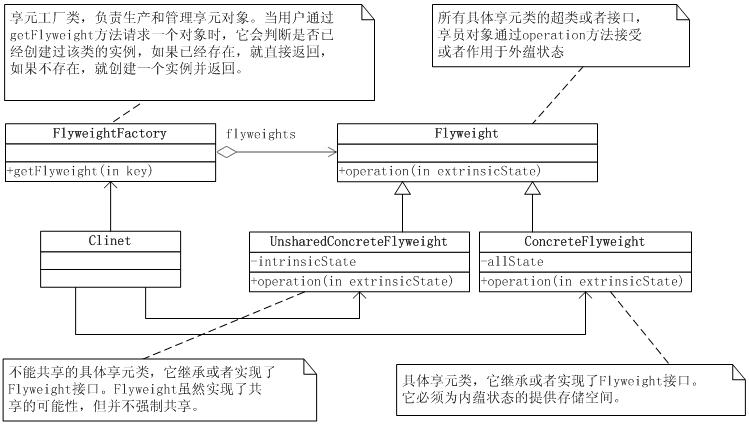
\includegraphics[scale= 0.8]{FlyWeight.png}
				\caption{FlyWeight Pattern}
				\label{FlyWeight}
			\end{figure}
		
		\begin{enumerate}[itemindent = 1em]
			\item 	\textbf{抽象享元类(Flyweight)}:	它是所有具体享元类的超类。为这些类规定出需要实现的公共接口,那些需要外蕴状态(Exte的操作可以通过方法的参数传入。抽象享元的接口使得享元变得可能,但是并不强制子类实行共享,因此并非所有的享元对象都是可以共享的。
				
			\item 	\textbf{具体享元类(ConcreteFlyweight)}:具体享元类实现了抽象享元类所规定的接口。如果有内蕴状态的话,必须负责为内蕴状态提供存储空间。享元对象的内蕴状态必须与对象所处的周围环境无关,从而使得享元对象可以在系统内共享。有时候具体享元类又称为单纯具体享元类,因为复合享元类是由单纯具体享元角色通过复合而成的。
			
			\item 	\textbf{不能共享的具体享元类(UnsharableFlyweight)}:不能共享的享元类,又叫做复合享元类。一个复合享元对象是由多个单享元对象组成,这些组成的对象是可以共享的,但是复合享元类本身并不能共享。
			
			\item 	\textbf{享元工厂类(FlyweightFactoiy)}:享元工厂类负责创建和管理享元对象。当一个客户端对象请求一个享元对象的时候,享元工厂需要检查系统中是否已经有一个符合要求的享元对象,如果已经有了,享元工厂角色就应当提供这个已有的享元对象;如果系统中没有适当的享元对象的话,享元工厂角色就应当创建一个新的合适的享元对象。
			
			\item   \textbf{客户类(Client)}:客户类需要自行存储所有享元对象的外蕴状态。
		\end{enumerate}	
		
	\subsection{实现}
		\begin{lstlisting}
	class Character    
	{  
		public:  
		virtual ~Character(){};  
		
		virtual void SetSize(int, int) = 0;  
		virtual void Display() = 0;  
		protected:  
		Character(){};  
		char m_chSymbol;  
		int m_nWeight;  
		int m_nHeight;  
	};  
	
	class CharacterA : public Character  
	{  
		public:  
		CharacterA();  
		virtual ~CharacterA();  
		
		void SetSize(int, int);  
		void Display();  
	};  
	
	class CharacterB : public Character  
	{  
		public:  
		CharacterB();  
		virtual ~CharacterB();  
		
		void SetSize(int, int);  
		void Display();  
	};  
	
	class CharacterFactory    
	{  
		public:  
		CharacterFactory()
		{
			m_mChar.insert(make_pair<char, Character*>('A', new CharacterA));  
			m_mChar.insert(make_pair<char, Character*>('B', new CharacterB)); 
		}
		virtual ~CharacterFactory();  
		
		Character* GetCharacter(char)
		{
			map<char, Character*>::iterator it = m_mChar.find(chIn);  
			if(it != m_mChar.end())  
			{  
				return (Character*)it->second;  
			}  
			
			return NULL; 
		}
		private:  
		std::map<char, Character*> m_mChar;  
	};  
	
	//// 享元模式 分离变化 与 管理分享同属性的多个对象 ////////
	int _tmain(int argc, _TCHAR* argv[])  
	{  
		CharacterFactory* pFactory = new CharacterFactory;  
		
		//内蕴状态 存储在享元对象内部并且不会随环境改变而改变  
		Character* ch1 = pFactory->GetCharacter('A');  
		ch1->Display();  
		
		//外蕴状态 客户端保存  
		Character* ch2 = pFactory->GetCharacter('B');  
		ch2->SetSize(500, 800);  
		ch2->Display();  
		return 0;  
	}  
		\end{lstlisting}	
	\subsection{应用场景}	
		\begin{itemize}
			\item Flyweight采用对象共享的做法来降低系统中对象的个数,从而降低细粒度对象给系统带来的内存压力。
			\item 当系统中有大量的细粒度对象实例,而且这些对象实例中有一些属性是重复的情况下,考虑使用
		\end{itemize}
		
		享元模式的优点在于\textbf{它大幅度地降低内存中对象的数量}。但是,它做到这一点所付出的代价也是很高的:\textbf{享元模式使得系统更加复杂}。为了使对象可以共享,需要将一些状态外部化,这使得程序的逻辑复杂化。另外它将享元对象的状态外部化,而读取外部状态使得运行时间稍微变长。
		
	\subsection{参考}
		\url{http://blog.csdn.net/lcl_data/article/details/8974679}

\newpage
\section{*适配器模式 Adapter-接口隔离}
	适配器模式把一个类的接口变换成客户端所期待的另一种接口,从而使原本接口不匹配而无法在一起工作的两个类能够在一起工作。比如说我的hp笔记本,美国产品,人家美国的电压是110V的,而我们中国的电压是220V,要在中国能使用,必须找个变压器转一下电压才可以。这个变压器就是个适配器。
	适配器模式有类适配器和对象适配器两种模式
	
	\subparagraph{结构:}Adapter 的典型结构图如下图\ref{Adapter}:
	\begin{figure}[h]
		\centering
		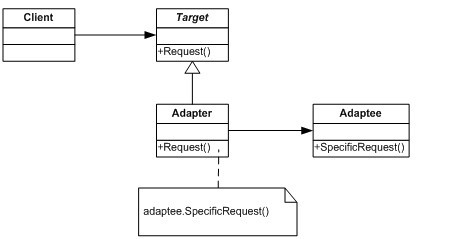
\includegraphics[scale= 1]{Adapter1.png}
		\caption{Class Adapter Pattern}
		\label{Adapter}
	\end{figure}
	
	\begin{figure}[h]
		\centering
		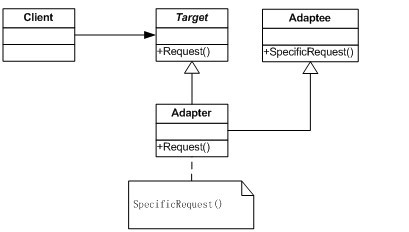
\includegraphics[scale= 1]{Adapter2.png}
		\caption{Object Adapter Pattern}
		\label{Adapter2}
	\end{figure}
	
	\subsection{实现}
		\begin{lstlisting}
	// Class Adapter Implementation
	// "ITarget"  
	class Target  
	{  
		public:  
		// Methods  
		virtual void Request(){};  
	};  
	
	// "Adaptee"  
	class Adaptee  
	{  
		public:  
		// Methods  
		void SpecificRequest()  
		{  
			cout<<"Called SpecificRequest()"<<endl;  
		}  
	};  
	
	// "Adapter"  
	class Adapter : public Adaptee, public Target  
	{  
		public:  
		// Implements ITarget interface  
		void Request()  
		{  
			// Possibly do some data manipulation  
			// and then call SpecificRequest    
			this->SpecificRequest();  
		}  
	};  
	
	
	int main()  
	{  
		// Create adapter and place a request  
		Target *t = new Adapter();  
		t->Request();  
		
		return 0;  
	}  
	
	// Object Adapter Implementation/////////////////
	
	// "ITarget"  
	class Target  
	{  
		public:  
		// Methods  
		virtual void Request(){};  
	};  
	
	// "Adaptee"  
	class Adaptee  
	{  
		public:  
		// Methods  
		void SpecificRequest()  
		{  
			cout<<"Called SpecificRequest()"<<endl;  
		}  
	};  
	
	// "Adapter"  
	class Adapter : public Target  
	{  
		private:  
		Adaptee *adaptee;  
		
		public:  
		Adapter()  
		{  
			adaptee = new Adaptee();  
		}  
		
		// Implements ITarget interface  
		void Request()  
		{  
			// Possibly do some data manipulation  
			// and then call SpecificRequest    
			adaptee->SpecificRequest();  
		}  
	};  
	
	
	int main()  
	{  
		// Create adapter and place a request  
		Target *t = new Adapter();  
		t->Request();  
		
		return 0;  
	}  
		\end{lstlisting}
	\subsection{实现要点}
		\begin{itemize}
			\item Adapter模式主要应用于“希望复用一些现存的类,但是接口又与复用环境要求不一致的情况”,在遗留代码复用、类库迁移等方面非常有用。
			
			\item Adapter模式有对象适配器和类适配器两种形式的实现结构,但是类适配器采用“\textbf{多继承”的实现方式,带来了不良的高耦合,所以一般不推荐使用}。对象适配器采用“对象组合”的方式,更符合松耦合精神。
			
			\item Adapter模式本身要求我们尽可能地使用“面向接口的编程”风格,这样才能在后期很方便的适配
		\end{itemize}
	\subsection{参考}
		\url{http://blog.csdn.net/lcl_data/article/details/8780140}
		

\newpage
\section{代理模式 Proxy -接口隔离}
	为其他对象提供一种代理以控制对这个对象的访问。
	
	\subparagraph{结构:}Proxy 的典型结构图如下图\ref{Proxy}:
	\begin{figure}[h]
		\centering
		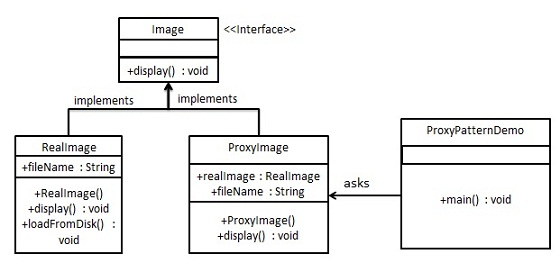
\includegraphics[scale= 0.7]{Proxy.jpg}
		\caption{Proxy Pattern}
		\label{Proxy}
	\end{figure}
	
	\begin{enumerate}[itemindent = 1em]
		\item \textbf{Subject}:定义RealSubject和Proxy的\textbf{共用接口},这样就可以\textbf{在任何使用RealSubject的地方都可以使用Proxy}
		\item \textbf{Proxy}:
			\begin{itemize}
				\item 提供一个与Subject的接口相同的接口,这样代理就可以用来代替实体,它的接口实际上可能只是实体接口的一个子集
				\item 保存一个引用使得代理可以访问实体
				\item 控制对实体的存取,并可能负责创建和删除它
			\end{itemize}
		\item RealSubject:定义Proxy所代表的实体
	\end{enumerate}	
	
	\subsection{实现}
		\begin{lstlisting}[language = java]
	public interface Image {
		void display();
	}
	
	public class RealImage implements Image {
	
		private String fileName;
		
		public RealImage(String fileName){
			this.fileName = fileName;
			loadFromDisk(fileName);
		}
		
		@Override
		public void display() {
			System.out.println("Displaying " + fileName);
		}
		
		private void loadFromDisk(String fileName){
			System.out.println("Loading " + fileName);
		}
	}
	
	public class ProxyImage implements Image{
	
		private RealImage realImage;
		private String fileName;
		
		public ProxyImage(String fileName){
			this.fileName = fileName;
		}
		
		@Override
		public void display() {
			if(realImage == null){
				realImage = new RealImage(fileName);
			}
			realImage.display();
		}
	}
	
	// 当被请求时,使用 ProxyImage 来获取 RealImage 类的对象
	public class ProxyPatternDemo {
	
		public static void main(String[] args) {
			Image image = new ProxyImage("test_10mb.jpg");
			
			//图像将从磁盘加载
			image.display(); 
			System.out.println("");
			//图像将无法从磁盘加载
			image.display(); 	
		}
	}
		\end{lstlisting}
\newpage
\section{外观模式 Facade -接口隔离}	


\chapter{行为模式-11种}
\section{*观察者模式 Observer -组件协作模式}
	\subsection{概要}
		有时被称作发布/订阅模式,观察者模式定义了一种\textbf{一对多的依赖关系},\textit{让多个观察者对象同时监听某一个主题对象。这个主题对象在状态发生变化时,会通知所有观察者对象,使它们能够自动更新自己}。
		
		\subparagraph{解决的问题:}将一个系统分割成一个一些类相互协作的类有一个不好的副作用,那就是需要维护相关对象间的一致性。我们不希望为了维持一致性而使各类紧密耦合,这样会给维护、扩展和重用都带来不便。观察者就是解决这类的耦合关系的
		
		\subparagraph{结构:}Observer 的典型结构图如下图\ref{Observer}:
		\begin{figure}[h]
			\centering
			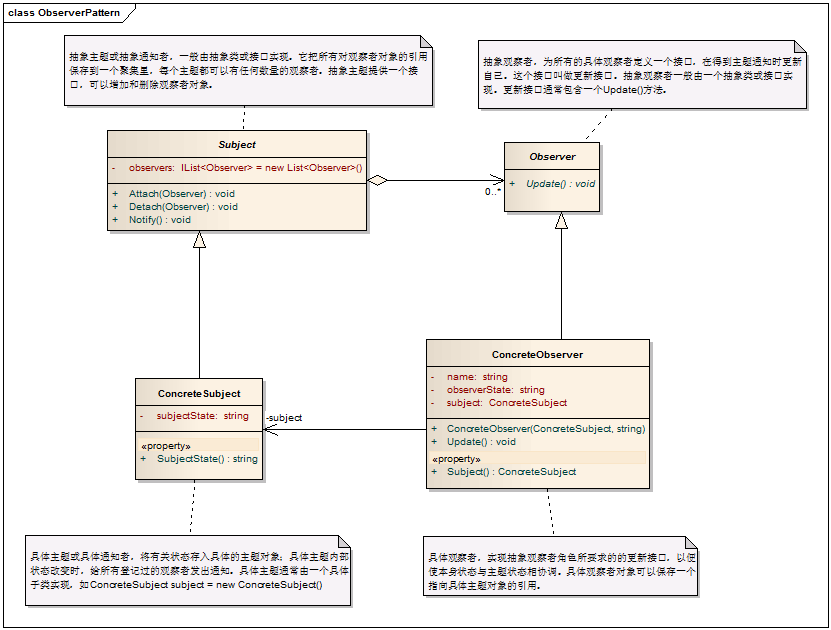
\includegraphics[scale= 0.7]{Observer.png}
			\caption{Observer Pattern}
			\label{Observer}
		\end{figure}
		
		\begin{enumerate}[itemindent = 1em]
			\item 抽象主题(Subject):它把\textbf{所有观察者对象的引用}保存到一个聚集里,\textbf{每个主题都可以有任何数量的观察者}。抽象主题提供一个接口,可以增加和删除观察者对象。
			\item 具体主题(ConcreteSubject):将有关状态存入具体观察者对象;\textit{在具体主题内部状态改变时,给所有登记过的观察者发出通知。}
			\item 抽象观察者(Observer):为所有的具体观察者定义一个接口,在得到主题通知时更新自己。
			\item 具体观察者(ConcreteObserver):实现抽象观察者角色所要求的更新接口,以便使本身的状态与主题状态协调。
		\end{enumerate}

	\subsection{实现}	
\begin{lstlisting}
	// Observer :观察者接口///////////////////////////////////
	class Observer
	{
	public:
		//得到观察主题 通知时,更新自己
		virtual void Update() = 0;
	
		virtual ~Observer(){}
	};
	
	// Subject: 观察的主题/////////////////////////////////////
	class Subject
	{
	public: 
		// 添加观察者
		virtual void AddObserver(Observer* observer) = 0;
		// 删除观察者
		virtual void RemoveObserver(Observer* observer) = 0;
		// 通知:变化了或更新
		virtual void Notify() = 0;
	
	private:
		list<Observer*> AllObservers;
	};
\end{lstlisting}
		\subsection{参考}
			\url{http://www.cnblogs.com/wangjq/archive/2012/07/12/2587966.html}
			
\newpage
\section{模版方法模式 -组件协作模式}

\newpage
\section{*策略模式 Strategy -组件协作模式}
	\subsection{概要}它定义了一系列的算法,并将每一个算法封装起来,而且使它们还可以相互替换。策略模式让算法的变化不会影响到使用算法的客户。
	
	\subparagraph{结构:}Strategy 的典型结构图如下图\ref{Strategy}:
	\begin{figure}[h]
		\centering
		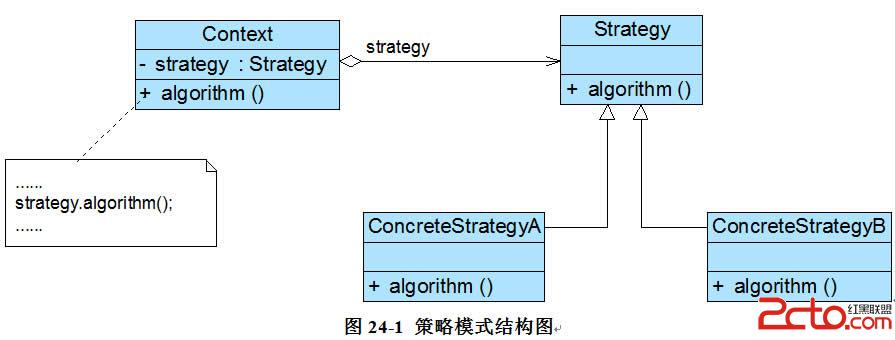
\includegraphics[scale= 0.7]{Strategy.jpg}
		\caption{Strategy Pattern}
		\label{Strategy}
	\end{figure}
	
		\begin{enumerate}[itemindent = 1em]
			\item 抽象策略: 1个
			\item 具体策略多个,封装了相关的算法和行为
			\item 调度类: 持有一个具体策略类的引用,供客户端使用
		\end{enumerate}
		
	\subsection{实现}
		\begin{lstlisting}
	#include<iostream>
	using namespace std;
	/*************************************策略基类****************************************/
	
	class StrategyBase//主要定义了虚函数
	{
		public:
		virtual void multiWay_tour()=0;//说明是纯虚函数(没有实现的虚函数),必须如此声明
	};
	
	/*************************************具体策略类****************************************/
	
	class StrategyFirstChild:public StrategyBase//策略子类,主要对父类定义的虚方法进行具体实现
	{
		public:
		void multiWay_tour()
		{
		cout<<"I'll go tourism on feet"<<endl;
		}
	};
	
	class StrategySecondChild:public StrategyBase//策略子类,主要对父类定义的虚方法进行具体实现
	{
		public:
		void multiWay_tour()
		{
		cout<<"I'll go tourism by train"<<endl;
		}
	};
	
	/*************************************调度类****************************************/
	
	class Context //调度类,根据传进来的参数,选择具体某个策略----待优化<参考教程>
	{
		private:
		StrategyBase *strategyChild;
		
		public:
		Context(StrategyBase *child)
		{
		strategyChild=child;
		}
		void multiWay_tour()
		{
		strategyChild->multiWay_tour();
		}
	
	};
	
	/*************************************客户端****************************************/
	int main()
	{
		cout<<"测试程序"<<endl;
		
		//“具体策略类”只在定义多个“调度类”时使用
		Context *Context_A=new Context(new StrategyFirstChild()),
		*Context_B=new Context(new StrategySecondChild()),
		*Context_C=new Context(new StrategySecondChild());
		
		//调用方法,只通过“调度类”实现,算法之间的差异已被屏蔽
		Context_A->multiWay_tour();
		Context_B->multiWay_tour();
		Context_C->multiWay_tour();
		
		cout<<endl;
		return 0;
	}
		\end{lstlisting}
		
		\subsection{应用场景}
			根据不同的情况,创建不同的对象.对象不同类型相近,方法差别大. 尤其适合经常变动的多种不同算法。 一般用于多个类的方法名都相同,但是实现方式不同
			
			\textbf{注重多个对象的\underline{相同行为}}:\textit{屏蔽方法名相同,算法实现细节不同之间的差异}(eg:txt、xml、dat、access四种格式的数据操作,读取,删除,修改)
			
			
\newpage
\section{状态模式 -状态变化}

\newpage
\section{备忘录模式 -状态变化}

\newpage
\section{中介者模式 -接口隔离}

\newpage
\section{命令模式 -行为变化模式}

\newpage
\section{访问者模式 -行为变化模式}

\newpage
\section{职责链模式 -数据结构模式}

\newpage
\section{*迭代器模式 Iterator-数据结构模式}
	\subsection{概要}
		在现在的电视机中,我们使用[后一个]和[前一个]按钮可以很方便的换台,当按下[后一个]按钮时,将切换到下一个预置的频道。想象一下在陌生的城市中的旅店中看电视。当改变频道时,重要的不是几频道,而是节目内容。如果对一个频道的节目不感兴趣,那么可以换下一个频道,而不需要知道它是几频道。
		
		这个其实就是我们\textbf{迭代器模式的精髓}:\textbf{提供一种方法顺序访问一个聚合对象中各个元素, 而又不需暴露该对象的内部表示}。
	
		\subparagraph{结构:}Iterator 的典型结构图如下图\ref{Iterator}:
		\begin{figure}[h]
			\centering
			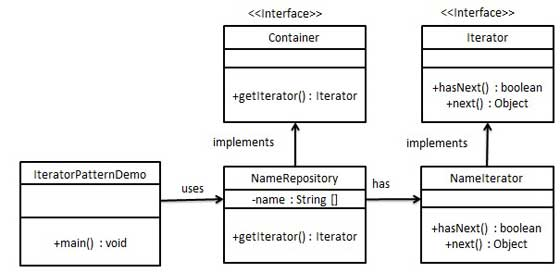
\includegraphics[scale= 0.7]{Iterator.jpg}
			\caption{Iterator Pattern}
			\label{Iterator}
		\end{figure}
		
			\begin{enumerate}[itemindent = 1em]
				\item \textbf{迭代器角色(Iterator)}:迭代器角色负责定义访问和遍历元素的接口。
				\item \textbf{集合角色(Aggregate)}:集合角色负责提供创建具体迭代器角色的接口。
				\item \textbf{具体集合角色(Concrete Aggregate)}:具体集合角色实现创建具体迭代器角色的接口——这个具体迭代器角色于该集合的结构相关。
				\item \textbf{集合角色(Aggregate)}:集合角色负责提供创建具体迭代器角色的接口
			\end{enumerate}
	\subsection{实现}
		\begin{lstlisting}
	template<class Item>
	class Iterator
	{
		public:
		virtual void first()=0;
		virtual void next()=0;
		virtual Item* currentItem()=0;
		virtual bool isDone()=0;
		virtual ~Iterator(){}
	};
	
	template<class Item>
	class Aggregate			// 类图中的Container
	{
		public:
		virtual Iterator<Item>* createIterator()=0;
		virtual ~Aggregate(){}
	};
	
	template<class Item>
	class ConcreteAggregate:public Aggregate<Item>	// 类图中具体类型的Container
	{
		vector<Item >data;
		public:
		ConcreteAggregate()
		{
			data.push_back(1);
			data.push_back(2);
			data.push_back(3);
		}
		virtual Iterator<Item>* createIterator()
		{
			return new ConcreteIterator<Item>(this);
		}
		Item& operator[](int index)
		{
			return data[index];
		}
		int getLen()
		{
			return data.size();
		}
	};	
	
	template<class Item>
	class ConcreteIterator : public Iterator <Item>	// 具体类型的迭代器
	{
		ConcreteAggregate<Item> * aggr;
		int cur;
		public:
		ConcreteIterator(ConcreteAggregate<Item>*a):aggr(a),cur(0){}
		virtual void first()
		{
			cur=0;
		}
		virtual void next()
		{
			if(cur<aggr->getLen())
				cur++;
		}
		virtual Item* currentItem()
		{
			if(cur<aggr->getLen())
				return &(*aggr)[cur];
			else
				return NULL;
		}
		virtual bool isDone()
		{
			return (cur>=aggr->getLen());
		}
	};
	

	
	int main()
	{
		Aggregate<int> * aggr =new ConcreteAggregate<int>();
		Iterator<int> *it=aggr->createIterator();
		
		for(it->first();!it->isDone();it->next())
		{
			cout<<*(it->currentItem())<<endl;
		}
		delete it;
		delete aggr;
		return 0;
	}
		\end{lstlisting}
	\subsection{参考}
		\url{http://blog.csdn.net/lcl_data/article/details/9310313}

\newpage
\section{解释器模式 -领域问题}




\chapter{UML 篇}
\section{类图符号}
	UML 中,可见性分为4级
	\begin{enumerate}[itemindent = 1em]
		\item \textbf{public}:	用 \textbf{+} 前缀表示 ,该属性对所有类可见
		\item \textbf{protected}:用\textbf{\#} 前缀表示,对该类的子孙可见
		\item \textbf{private}:	用 \textbf{-} 前缀表示 ,只对该类本身可见
		\item \textbf{package}:	用 \textbf{$\sim$} 前缀表示,只对同一包声明的其他类可见
	\end{enumerate}

	\begin{figure}[h]
		\centering
		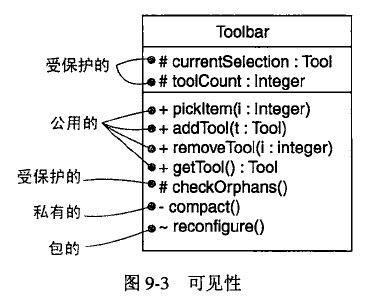
\includegraphics[width = 9cm]{Simbol_UML.jpg}
	\end{figure}
	
	All:\url{http://blog.csdn.net/caozhangyingfei0109/article/details/8534191}
\newpage

\section{类图关系}
	\begin{enumerate}
		\item \textbf{继承}:指的是一个类(称为子类、子接口)继承另外的一个类(称为父类、父接口)的功能,并可以增加它自己的新功能的能力,继承是类与类或者接口与接口之间最常见的关系;
			\begin{figure}[h]
				\centering
				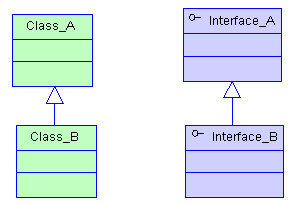
\includegraphics[scale = 0.7]{DeriveShip.jpg}
				\caption{继承}
			\end{figure}
		\item \textbf{依赖}:可以简单的理解,就是一个类A使用到了另一个类B,而这种使用关系是具有偶然性的、、临时性的、非常弱的,但是B类的变化会影响到A;比如某人要过河,需要借用一条船,此时人与船之间的关系就是依赖;表现在代码层面,为类B作为参数被类A在某个method方法中使用;
			\begin{figure}[h]
				\centering
				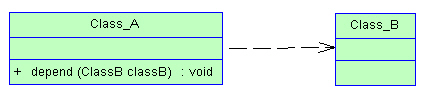
\includegraphics[scale = 0.7]{DependShip.jpg}
				\caption{依赖}
			\end{figure}
		\item \textbf{关联}:他体现的是两个类、或者类与接口之间语义级别的一种强依赖关系,比如我和我的朋友;这种关系比依赖更强、不存在依赖关系的偶然性、关系也不是临时性的,一般是长期性的,而且双方的关系一般是平等的、关联可以是单向、双向的;表现在代码层面,为被关联类B以类属性的形式出现在关联类A中,也可能是关联类A引用了一个类型为被关联类B的全局变量;
			\begin{figure}[h]
				\centering
				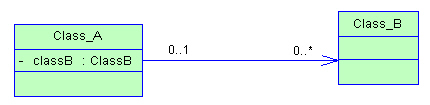
\includegraphics[scale = 0.7]{Association.jpg}
				\caption{关联}
			\end{figure}
		\item \textbf{聚合}:聚合是关联关系的一种特例,他体现的是整体与部分、拥有的关系,即has-a的关系,此时整体与部分之间是可分离的,他们可以具有各自的生命周期,部分可以属于多个整体对象,也可以为多个整体对象共享;比如计算机与CPU、公司与员工的关系等;表现在代码层面,和关联关系是一致的,只能从语义级别来区分; 
			\begin{figure}[h]
				\centering
				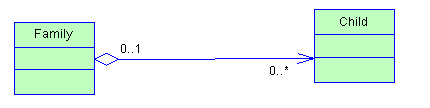
\includegraphics[scale = 0.7]{Aggregation.jpg}
				\caption{聚合}
			\end{figure}
		\item \textbf{组合}:组合也是关联关系的一种特例,他体现的是一种contains-a的关系,这种关系比聚合更强,也称为强聚合;他同样体现整体与部分间的关系,但此时整体与部分是不可分的,整体的生命周期结束也就意味着部分的生命周期结束;比如你和你的大脑;表现在代码层面,和关联关系是一致的,只能从语义级别来区分; 
			\begin{figure}[h]
				\centering
				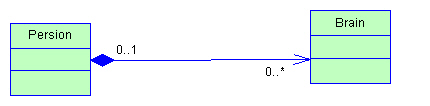
\includegraphics[scale = 0.7]{Composition.jpg}
				\caption{组合}
			\end{figure}
	\end{enumerate}

\section{时间序列图}


\section{包图}


\end{document} 
